        % Chapter 1

\chapter{Summative Evaluation} % Main chapter title

\label{summativeevalchapter} % For referencing the chapter elsewhere, use \ref{Chapter1} 

\lhead{Chapter \ref{summativeevalchapter}. \emph{Summative Evaluation}} % This is for the header on each page - perhaps a shortened title

%----------------------------------------------------------------------------------------
\section{Recruitment of Participants}
With help of a research assistant who was a resident of Langa,  we managed to recruit a total of fourteen adult participants (beneficiary users) through convenient sampling. Approaching of potential participants for recruitment was done in October 2015. We recruited these participants from two townships in Cape Town: Langa, and Athlone. In Langa there were five adult participants while in Athlone there were nine adult participants. The average age of these adult participants was 44.21 years with a standard deviation (S.D) of 9.99 years. The youngest adult was 26 years of age while the oldest was 60 years of age. Thirteen participants were females. The reason for this gender imbalance is that women were more eagerly to participate compared to men during recruitment. We have already seen this trend even in the study reported in Chapter \ref{prototytpe2chapter}.

Majority of the adult participants had a maximum education level of either grade 7 of primary school or grade 12 of secondary school. Each adult participant (beneficiary user) elected one of their children/grand children to become their respective intermediary user; hence forming a pair of users. Therefore, there were a total of 14 pairs of users. The two members of a pair were required to work together in using the ``Family Wellness App'' to self-monitor diet and physical activity of an adult member of a pair (a beneficiary participant). As the result of pairing, thirteen beneficiary participants  were working with their children, while the remaining one was working with her grand child. The average age of children participants (intermediary users) was 15.42 (S.D=2.06) years. The youngest intermediary user was 12 years of age while the oldest was 20 years of age. The number of females and males intermediary users were equal. Both intermediary users were school going children at primary and secondary school levels.

I gave out detailed information of what the study was all about to both intermediary and beneficiary participants. I informed them about their different modes of which I will collect data such as logs, questionnaires, and interviews. All the beneficiary participants signed informed consent forms agreeing to be part of the study. Since all intermediaries were under 21 years of age (legal age for giving consent in South Africa is 21 and above), they signed assent forms which were also signed by their respective parents/guardians who were part of the study.

One day was allocated for training intermediary participants on how to use the ``Family Wellness App''. In addition, each intermediary user was given a user manual. After the training, I gave out one Android phone (Samsung GT-S5300) to each pair of participants. These phones were installed with two natives apps. The first app was a pedometer and the second one was the main ``Family Wellness App''. The ``Family Wellness App'' loaded all its content from a web application hosted remotely at University of Cape Town servers. Each beneficiary participants was required to carry the experiment phone with them all the time in order for the pedometer app to count their footsteps. The two apps (main app and pedometer) were made available to the pairs of participants for a total period of six weeks. Each pair of participants provided the service provider's number of the SIM card that was inserted on their given Android phone. I allocated 1.3 GB of data to each SIM card. In addition each beneficiary participant was given a total of ZAR 240 for the duration of the study. The amount covered for compensation for participants' transportation and time for points where there data collection activities such as administering of questionnaires and interviews. The details of the experiments are outlined on the next section. 
\section{Experiments}
This phase of the study evaluated the effectiveness of gamification/rewards in motivating  intermediaries to collaborate with their respective beneficiaries in order to utilize the ``Family Wellness App''. I was comparing two versions of the applications. The first version of the application was simply a logbook or journal that allows each pair of users (1) to record and view diet/nutritional data of the beneficiary member of the pair, and (2) to view progress in accumulation of footsteps of a beneficiary member of the pair. The second version of the application was an extension of logbook meaning that it included all the feature in logbook  with an addition of a rewards/gamified subsystem. The experiments took place from the mid-October 2015 to the end of November 2015.  The details of how experiments were designed and how data were collected are presented on the next sub-section.
\subsection{Experiment Design}
The study used ``within-group'' design for the experiments. In within-group design, the same group of participants were exposed to different experimental conditions. This helps to minimize the number of groups needed to test hypotheses as only one group is used for both control and intervention. Another advantage of within-group design is that it minimizes the effect of confounding factors. The only problem with this approach is the learning effect and in addition, it lengthens duration of a study. In order to minimize the impact of the learning effect on the outcome, I randomly assigned pairs of participants to two separate groups referred to as experimental sequences. The first experimental sequence started with the \emph{logbook app}  and finished with the \emph{gamified} app. The second experimental sequence started with the \emph{gamified app} and finished with the ``logbook app''. I used the following abbreviations ``LG'' and ``GL'' to refer to respective first and second experimental sequences.

A total of seven pairs of participants were assigned to the LG group while the remaining seven pairs were assigned to the GL group. Both groups spent the first four weeks in their respective first experimental conditions of which were logbook app for the LG group and gamified app for the GL group. After 27 days (four weeks) each group was switched to a different experimental condition; hence after the switching, the LG group started using the gamified app while the GL group started using the logbook app. The second phase of the experiment lasted for a total of 14 days (two weeks). 

The explanation of why four weeks in phase 1 and two weeks in phase 2 is as follows. Initially the plan was to have time spent on each experimental condition, be in three(3) weeks intervals, but phase 1 had extended beyond it allocated block of three weeks up to the fourth week as pairs of participants were not available for midpoint assessments at the end of the third week. Therefore, the midpoint assessment was carried out at the end of the fourth week. After the aforementioned assessment, pairs that were in gamified app were switched to logbook app, and those that were in logbook app were switched to gamified app. It was not feasible to extend phase 2 to go up to four weeks as phase 1 due complexity that was going to be introduced as the result of rescheduling duration of experiments from six to eight weeks. Rescheduling was impossible because it was approaching December of where most people travel for holidays, therefore, gathering participants during that time may have been impractical. As the result this shortened the duration of phase 2 to two weeks.
\subsection{Data Collection Methods and Analysis}
Data collection was a triangulation of application's logs,questionnaires and interviews. 
\subsubsection{Family Wellness App Logs}
Application's logs consisted of information regarding the time when there were users' activities on the app, the pair that was accessing the app at that time, and the functionality that was being accessed by that pair. Logs were categorized to their respective experimental conditions. Usage was characterized by two dimensions: (1) the number of sessions of where the app had user activity from a particular pair of users, and (2) the number of times certain features were accessed by a particular pair of users. A new session was defined as a period of detection of user's activity in an absence of any activity from this user/pair in the past one hour or more. The number of times in which a certain feature was accessed was defined as the period of detection of user's/pair's usage activity on a certain feature in an absence of any of their usage activity on that particular feature in the past one minute or more, therefore, if clicks are within an interval one minute on the same feature, it means the user is still on the same feature they had opened last time and they have not moved away from that feature since then. If the time difference between clicks is beyond one minute, then it was assumed that the user had gone away or move to a different feature and they are coming to this feature for another iteration of clicks on the feature as the previous iteration of clicks within the that feature they are visiting had finished. The aim of this dimension was to understand where users of the app were likely to go among options of gamification features which were score board (leader board), score badge, botanical garden, and fish tank (fish aquarium). 
 
I carried out comparison of number of sessions between gamified app and logbook in two sub-dimensions. The first comparison entailed comparing the daily total number of sessions between the two experimental conditions for 41 days of experiments. This was the comparison between daily total of all sessions of users in logbook app and daily total of all sessions   of users in gamified app.

In the second comparison, it was a pairwise comparison of users' sessions in between logbook and gamification conditions. In order to ensure this comparison of usage doesn't get affected by differing lengths of experimental durations between experimental conditions, I opted to use a relative (normalized) number of sessions  as a unit of measurement. In this case I used the number of sessions per day since the number of sessions on a particular experimental condition was relative to the number of days on which a particular version of the app was made available to the pair of users. This number differed between experimental conditions within the same experimental sequence (group). For instance the LG group spent nearly four weeks in logbook app and only two weeks in the gamified app while the GL group spent two weeks in logbook app and four weeks in gamified app. This implies if a pair that belongs to an experimental group (sequence), \emph{Z} spent an \emph{X} amount of days in an experimental condition \emph{Y} and had \emph{n} number of sessions, then their normalized number of sessions in experimental condition \emph{Y} will be \emph{\textbf{n}} sessions divide by \emph{\textbf{X}} days. In the process of doing this comparison, I made a decision to exclude four pairs from analysis. These were pairs that faced hurdles on utilizing the app as the result of technical glitches and this affected their ability to fully experience and engage with what was being offered by the two versions of the family wellness app. These pairs are listed on Table \ref{table:usageproblems}.
\begin{table}[h!]
  \begin{center}
    \caption{Pairs with usability/technical problems that hinder their participation}
    \label{table:usageproblems}
	\begin{tabular}{|l|l|l|p{6cm}|}
		\hline
		&Pair&Experimental Sequence&Problem\\
		\hline
		1&Pair A&GL group &App not loading\\
		\hline
		2&Pair B&GL group&Lack of data bundles. \\
		\hline
		3&Pair C & LG group.& Pedometer never transmitted data to the server.\\
		\hline
		4&Pair D & LG group.& Pedometer stopped transmitting data to the server.\\
	\hline
	\end{tabular}
  \end{center}
\end{table}
For \textbf{Pair A}, the app failed to load every time the intermediary user tried to use it. An intermediary user from this pair complained that the app was unstable. After I made a follow up, I observed that in the house where that pair lived lived in there was a poor Internet signal, hence the app was always failing to load most of the time and this frustrated the intermediary. The second pair (\textbf{Pair B}), data was allocated to the wrong phone number at the beginning of experiments but they never reported on time. These two pairs (Pair A and Pair B) had the lowest usage days which were 2 and 3 days respectively and they they had used the app only in gamification condition.

For the last two pairs (\textbf{Pairs C} and \textbf{D}) on Table \ref{table:usageproblems}, their pedometers had malfunctioned; hence in Pair C, footsteps' data were never transmitted to the server while in Pair D the pedometer stopped transmitting data on the fourth week of experiments (before switching of experimental conditions). Both of these two pairs were in LG group meaning that they had started with logbook in phase 1 of experiments. Despite the technical glitches these pairs reported higher utilization of the app while in logbook condition compared to other pairs in logbook condition. In this context, intermediary users of the pairs were the main driver of utilization hence their engagement was crucial for sustainable utilization. It was expected that their usage will be even be higher once they were switched to gamification condition as it was for the case of other pairs that were switched from logbook to gamification as shown on Figure \ref{figure:lg_tech_prob_vs_w_o_tech_prob}. However, that was not the case as there was no incentive for them to sustain utilization of the app since the failure of the pedometer was coupled with the learning effect; therefore, it lowered their user experience and affected their utilization after being switched to gamification. Steps data were important in gamification condition for pairs of users to advance in badges and leaderboard points, and for improvement of both the fish tank and botanical garden.
 
\begin{figure}[htbp]
  \centering
    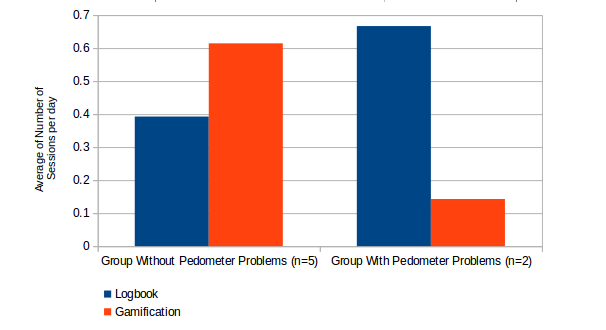
\includegraphics[width=0.6\textwidth]{Figures/compare_lg_problems_without_problems.png}
    \rule{35em}{0.5pt}
  \caption{Average of number of sessions per day for pairs in LG group with and without pedometer problems.}
  \label{figure:lg_tech_prob_vs_w_o_tech_prob}
\end{figure}

Friendship between the two intermediary users from Pair C and Pair D explained why there were so much similarities in their usage pattern while in logbook condition. Although the pedometer never transmitted data in Pair C  since the beginning of experiments, an intermediary user from this pair continued to use the family wellness app because of the informal comparison with an intermediary user from Pair D while they were both still in logbook condition. Their usage in Pair C and Pair D were both 11 days. Their drop out started during gamification condition. Pair C and Pair D used the app for three days and one day respectively. And that usage happened within the first week of starting to use gamification. Since gamification depended on transmission of steps to the server, pedometer problems affected Pair C and Pair D motivations to participate in gamification phase despite their efforts during logbook condition. The learning effect coupled with problems with their pedometers mediated their decrease in usage with the app. An intermediary user from another pair (let's called it Pair G) who was also part of the ``LG'' group happened to live nearby, was often interacting with intermediary users of Pair D and Pair C. This intermediary user from Pair G shared her concerns about the credibility of rewards offered by the gamified app. This was during the endline interviews. This particular intermediary user didn't appreciate her advancement in badges because she admitted that her peers (the two intermediary users from Pair C and Pair D) did more efforts than her but they were not getting anything so she didn't understand why she was ahead of them. She was referring to their usage during logbook condition as they were both using the ``logbook App'' at the same time.  This proves that usability problems played a role to the some extent in demotivating participation in gamification condition  of intermediary users from Pair C and Pair D. So to compare usage the hypothesis of interest is:

\begin{enumerate}
\item{Hypothesis 1}
\begin{itemize}
\item{H\SB{0}}:There is no difference in number of sessions between a logbook app and gamified app
\item{H\SB{A}}:There is a difference in number of sessions between a logbook app and gamified app
\end{itemize}
\end{enumerate}

The last analysis on usage logs examined the impact of gamification features on internalization. Perceived usefulness is a predictor of internalization. I devised a term called impressions which is the number of times in which a certain feature had been viewed. So if multiple views by one user/pair on one feature happened within an interval of less than one minute between consecutive views, such multiple consecutive views were treated as one impression. If views on same the same feature differed by a minute or more then each view was treated as one impression. Therefore, the total number of impressions on each of gamification feature was calculated for the number of days in which pairs were assigned to gamification condition. In this analysis we considered all fourteen pairs  including the four that had technical glitches. Since this comparison only involved one experimental condition; hence all features had equal chances of being accessed provided that the user has managed to get into the app. Also some feedbacks were delivered through SMS meaning that all pairs had received such interactions regardless of whether the App was accessible or not; therefore, it is under the assumption that pairs pairs that had received SMS feedback could be in position of judging the perceived usefulness of the app. In addition to that, intermediary users were frequently interacting to each other in face to face manner to talk about things in the app. Another assumption is that regardless of the app presence intermediary users would perceive helping their parents on app usage as something that as something that is meaningful. Hence if the user/pair had never viewed a particular gamification feature, they would still get zero as the number of impressions in that feature. The objective was to understand how gamification features affect internalization. On literature review section (Chapter \ref{literaturereview}), four types of internalization of behaviour regulation were highlighted. Therefore, this analysis also view internalization with respect to the four types of behaviour regulation. The questionnaires that were used to capture aspects of internalization (perceived useful) are mentioned on the next sub-section together with other sub-scales of intrinsic motivation.

\subsubsection{Questionnaires}\label{methodsquestionnaire}
The research team administered questionnaires at baseline, mid-line (during switching of experimental conditions), and end-line. These questionnaires targeted both intermediary and beneficiary participants. The list of questionnaires is provided below.
\begin{enumerate}
\item{\textbf{Intermediaries}}
Intermediaries had three questionnaires that were administered at baseline, midline, and endline.
 
\begin{itemize}
\item{\textbf{Baseline Questionnaire}}: Intermediaries participants' baseline questionnaire had three sections. The first section captured demographic information such as age,gender, and number services/apps used on cellphones.The second section included an IMI (Intrinsic Motivation Inventory) questionnaire  to assess participants' intrinsic motivation in using cellphones. The third section included an IMI questionnaire to assess participants' intrinsic motivation in helping their parents with cellphone based tasks. 

\item{\textbf{Midline Questionnaire}}: Intermediaries participants' midline questionnaire had only one section which included an IMI questionnaire  to assess participants' intrinsic motivation in using the family wellness app.

\item{\textbf{Endline Questionnaire}}: Intermediaries participants' endline questionnaire had only one section which included an IMI questionnaire  to assess participants' intrinsic motivation in using the family wellness app.
\end{itemize}

\item{\textbf{Beneficiaries}}

\begin{itemize}
\item{\textbf{Baseline Questionnaire}}: Beneficiary participants' baseline questionnaire had four sections. The first section included an IMI questionnaire  to assess participants' intrinsic motivation in using the family wellness app. The third section included an IMI questionnaire to assess participants' intrinsic motivation in self-monitoring of diet/nutrition. The fourth section included an IMI questionnaire to assess participants' intrinsic motivation in self-monitoring of physical activity.

\item{\textbf{Midline Questionnaire}}:Beneficiary participants' midline questionnaire had three sections. The first section included an IMI questionnaire  to assess participants' intrinsic motivation in using the family wellness app. The third section included an IMI questionnaire to assess participants' intrinsic motivation in self-monitoring of diet/nutrition.The fourth section included an IMI questionnaire to assess participants' intrinsic motivation in self-monitoring of physical activity.

\item{\textbf{Endline Questionnaire}}: Beneficiary participants' endline questionnaire had three sections. The first section included an IMI questionnaire  to assess participants' intrinsic motivation in using the family wellness app. The third section included an IMI questionnaire to assess participants' intrinsic motivation in self-monitoring of diet/nutrition.The fourth section included an IMI questionnaire to assess participants' intrinsic motivation in self-monitoring of physical activity.
\end{itemize}
\end{enumerate}

I developed the IMI questionnaires with the guidance of materials found on a ``Self-Determination Theory''\footnote{http://www.selfdeterminationtheory.org/intrinsic-motivation-inventory/} website which is maintained by researchers working on the theory including Richard Ryan and Edward Deci\citep{deci1985intrinsic} whom were early pioneers in developing the theory. I pretested these questionnaires during the informative evaluation of prototype II in chapter \ref{prototytpe2chapter}. The most important sub-scales for our theoretical construct were perceived competence and perceived autonomy which are part of the three basic psychological needs. The relatedness sub-scale is not yet validated but it was included in all questionnaires. Other sub-scales that were included all questionnaires or some of the questionnaires were perceived enjoyment, and perceived useful. Perceived enjoyment is the only direct measure of intrinsic motivation while perceived competence and perceived autonomy are predictors of intrinsic motivation. Self-Determination theory suggests that a behaviour can be started as externally motivated and if external motivators support the three basic psychological needs which are relatedness, competitiveness, and autonomy then a behaviour that was once externally motivated can be internalized and users will start doing it because it is a good thing to do. Perceived useful is a predictor of internalization.

In addition to the aforementioned sub-scales, perceived efforts also appears in specific questionnaires (i.e self-monitoring of diet and activity, use of cellphone). This additional sub-scale was included as part of the package of IMI questionnaire inventory as it may be directly linked to the important sub-scales. However, its results were of less interest to the theoretical constructs of this research.
  
The overall IMI scores were computed by averaging the scores from each sub-scales. In each question from the IMI sub scales, respondents were supposed to rate there experience in a scale of 1 to 7 points which means that 1 implies the statement is "not true at all" and 7 means the statement is "very true".

There were two main objectives of using the IMI questionnaire. The first objective was to assess the ability of the two prototypes in supporting the participants with the three basic psychological needs. The difference in experimental durations was expected not to have any effect on motivations to use either of the two systems since both logbook and gamification were both present in both phases of experiments. Therefore, effects on motivations due to different durations were expected to cancel each other during analysis. I compared between the capability of the two prototypes in affording three basic psychological needs suggested by self-determination theory. In addition, I also included perceptions on enjoyment as it is a direct measure of intrinsic motivation. The corresponding scales from the IMI questionnaire were administered at midline and endline . Therefore, there were four main sub-scales; perceived competence, perceived autonomy, perceived enjoyment and perceived relatedness. There were also one additional supporting sub scale which was perceived useful of which its purpose was to extract pattern on internalization as far as gamification features are concerned.

The second objective of using IMI questionnaires was to assess motivations/self-determinations of beneficiaries in self-monitoring of diet and activity, and motivation/self-determination to use cellphone of both intermediaries and beneficiaries. These IMI questionnaires included perceptions of beneficiaries on enjoyment, competence, autonomy, relatedness, enjoyment, effort, and usefulness.

The hypotheses of interest to both intermediaries and beneficiaries on intrinsic motivation's sub-scales related to usage of the app in different experimental conditions were:

\begin{enumerate}
 \setcounter{enumi}{1}
\item{Hypothesis 2}
\begin{itemize}
\item{H\SB{0}}:There is no difference in perceived competence in using the app between a logbook app and gamified app
\item{H\SB{A}}:There is a difference in perceived competence in using the app between a logbook app and gamified app.
\end{itemize}
\item{Hypothesis 3}
\begin{itemize}
\item{H\SB{0}}:There is no difference in perceived autonomy in using the app between a logbook app and gamified app
\item{H\SB{A}}:There is a difference in perceived autonomy in using the app between a logbook app and gamified app
\end{itemize}
\item{Hypothesis 4}
\begin{itemize}
\item{H\SB{0}}:There is no difference in perceived relatedness in using the app between a logbook app and gamified app
\item{H\SB{A}}:There is a difference in perceived relatedness in using the app between a logbook app and gamified app
\end{itemize}
\end{enumerate}

Each of the four aforementioned hypotheses was tested twice. The first test was to intermediary users' scores and the second on beneficiary users' scores. There were also hypotheses of interest for beneficiaries in self-monitoring of behaviours reported below:

\begin{enumerate}
 \setcounter{enumi}{4}
\item{Hypothesis 5}
\begin{itemize}
\item{H\SB{0}}:There is no difference in the overall self-determination to self-monitor diet of between a logbook app and gamified app
\item{H\SB{A}}:There is a difference in the overall self-determination to self-monitor diet of between a logbook app and gamified app
\end{itemize}
\item{Hypothesis 6}
\begin{itemize}
\item{H\SB{0}}:There is no difference in the overall self-determination to self-monitor activity of between a logbook app and gamified app
\item{H\SB{A}}:There is a difference in the overall self-determination to self-monitor activity of between a logbook app and gamified app
\end{itemize}
\end{enumerate}

In motivations to self-monitor diet and activity, I excluded pairs (A,B, C, and D) from Table \ref{table:usageproblems} with problems that led to discontinuation of usage. In total only ten out of fourteen beneficiaries had their results included for analysis in order to have only beneficiaries who had meaningful engagement with the app through their respective intermediaries. In the comparison for self-monitoring of diet and activity, the first IMI comparison  entailed comparing the IMI score of each participant at baseline, midline, and endline regardless of an experimental condition. In the second comparison I compared scores at baseline, and at both logbook and gamification conditions. The IMI score was computed from the average of all scores from sub-scales of perceived competence, perceived autonomy, perceived relatedness, perceived enjoyment, perceived effort,  and perceived usefulness. I  used one way ANOVA with repeated measures to test if there was a difference  between scores at: (1) baseline, midline, and endline, and (2)baseline, logbook and gamification. I used Mauchy's test\footnote{Read more on how Mauchy's test is used from http://www.statisticshell.com/docs/repeatedmeasures.pdf} to checked if different measuring points had the same covariance in each ANOVA test I carried out and this helped in deciding of whether to ``Sphericity Assumed'',``Greenhouse-Geisser'', or ``Huynh-Feldt'' of SPSS output.

Before each statistical test, samples were tested to find if they follow normal distribution``\emph{Shapiro-Wilk Normality Test}''\footnote{http://sdittami.altervista.org/shapirotest/ShapiroTest.html}) was used to test for normal distribution. For the case of paired samples, the difference between repeated measures of each data point was used to test for normality. In case there was no normality, I would apply a log transformation on the original data, and repeat the normality test again. If normality is achieved I would proceed into using statistical tests that assume normality such a t test with repeated measures or a one way ANOVA with repeated measures. In all cases of repeated measured, normality was achieved on the original data, as the result only statistical tests that assume a  normal distribution were used.  For the case of of independent samples, each sample was tested for normality. In the absence of a normal distribution in any of the two independent samples, a log transformation was applied in this context. There was a case of two independent samples where a log transformation couldn't result into any normal distribution, therefore, as the result, it was resorted to the use of a non-parametric test called Mann-Whitney U Test as will be reported on the findings. 
 
\subsubsection{Interviews}
I also conducted short unstructured interviews at midline and endline. I selected fewer intermediaries and beneficiaries for the interviews. Interviews responses were important in supplementing data collected through questionnaires and application's logs.
\section{Findings}
There were four primary outcomes in analysing the findings and these are: (1)usage trend of the app; (2) user experience/intrinsic motivation  of both intermediaries and intermediaries in using the app; (3) intrinsic motivation of beneficiaries in self-monitoring of diet/nutrition; and (4) intrinsic motivation of beneficiaries in self-monitoring of physical activity.
\subsection{Usage Outcome}
\label{usageoutcome}
\begin{figure}[htbp]
  \centering
    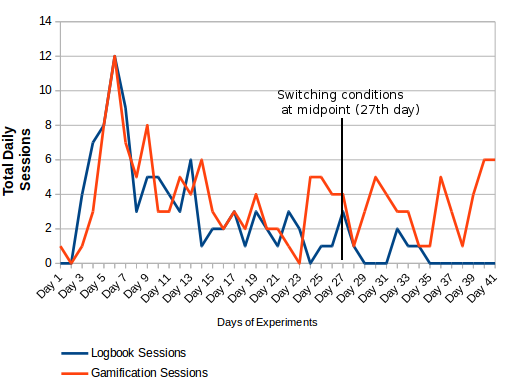
\includegraphics[width=0.6\textwidth]{Figures/scatter_daily_sessions.png}
    \rule{35em}{0.5pt}
  \caption{Total daily number of sessions from the two experimental conditions.}
  \label{figure:usagedailysessions}
\end{figure}
The average number of days on which pairs used both versions of the application was 10.5 (SD=7.39) days. The most active usage was from a pair that utilized the app for a total of 26 days. The less active usage was from a pair that had used the app for only two days out of 41 days. Figure \ref{figure:usagedailysessions} demonstrates trends on total daily usage's sessions in between logbook and gamification conditions. These trends indicate that in most days a gamified system had more total number of sessions compared to logbook. This is supported by a statistical comparison of daily total number sessions accumulated from all users in each experimental condition which showed that gamification condition had a significant total number of daily sessions compared to logbook as demonstrated by Mann-Whitney U Test on Table \ref{table:usagedays}.
\begin{table}[h!]
  \begin{center}
    \caption{Daily usage comparison between Logbook and Gamified systems for 41 days}
    \label{table:usagedays}
	\begin{tabular}{|L{3cm}|c|c|c|c|c|c|}
		\hline
		Groups&N&Rank Average&Sum Ranks&U&Z&P\\
		\hline
   		Daily logbook sessions&41&33.72&1701.5&\multirow{2}{*}{1159.5}&\multirow{2}{*}{-2.9538}& \multirow{2}{*}{0.00318}\\\cline{1-4} 
   		 		    Daily gamification sessions&41&49.28& 1701.5&&&\\
\hline
	\end{tabular}
  \end{center}
\end{table}

\begin{figure}[htbp]
  \centering
    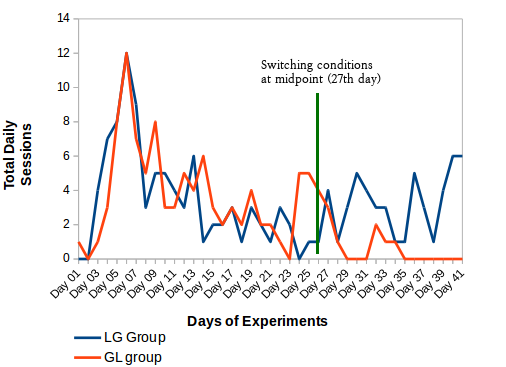
\includegraphics[width=0.6\textwidth]{Figures/usagedailysessions_lg_gl.png}
    \rule{35em}{0.5pt}
  \caption{Total daily number of sessions from the two experimental conditions.}
  \label{figure:usagedailysessions_lg_gl}
\end{figure}

An interesting phenomenon that expands on the usage pattern of Figure \ref{figure:usagedailysessions} above is that one of Figure \ref{figure:usagedailysessions_lg_gl} which shows usage trends of LG (logbook-gamification) and GL (gamification-logbook) groups. It can be observed that there is a sudden drop in number of usage sessions for users/pairs in GL group after being switched from gamification app to logbook app. This pattern suggests that most behaviour regulation during gamification condition was as the result of ego-involved (introjected regulation). This hypothesized situation is supported by a further exploration on number impressions on gamification features. On checking the average impressions among the four gamification, leaderboard seems to be having the highest average number of impressions as shown on Figure \ref{figure:gamification_impressions_latest_all}. 
\begin{figure}[htbp]
  \centering
    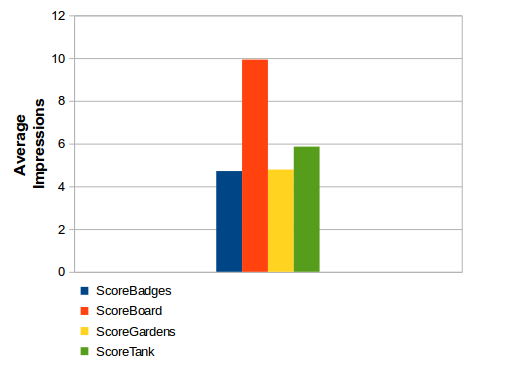
\includegraphics[width=0.6\textwidth]{Figures/gamification_impressions_latest_all.png}
    \rule{35em}{0.5pt}
  \caption{Total daily impressions for two groups (LG and GL).}
  \label{figure:gamification_impressions_latest_all}
\end{figure}
I conducted statistical comparison on the number of impressions between leaderboard and each of other gamification features (score badges, botanical garden, and fish tank). It was found that the number of impressions was statistically significant higher in leaderboard (M=9.93;SD=13.90) compared to score badges (M=4.71; SD=5.50) (t (13) =2.1747; p=0.0487). There was no statistical significance on either number of impressions between leaderboard (M=9.93; SD=13.90) and botanical garden (M=4.79; SD=5.26) (t(13)=1.716; p=0.1096) or number of impressions between leaderboard (M=9.93; SD=13.90) and fish tank (M=5.86; SD=7.40) (t(13)=1.5707; p=0.1403).However, the trend shows dominance of leaderboard over other gamification features. 

A further exploration on  gamification features' impressions reveals some insights on the trend of promotion of, ego involved, and task mastery, climates. This exploration follows the discussion of the previous chapter (Chapter \ref{prototytpe2chapter}) of where it was observed that some statements from qualitative feedback reflected that gamification features tended to promote either task mastery climate or ego-involved climate. In that previous discussion there was an indication that the leaderboard was likely to promote the ego-involved climate on some intermediary users while features like fish tank or botanical garden were likely to promote the task mastery climate. Literature suggests that promotion of task mastery climate may foster integrated internalization of behaviour regulation while promotion of ego-involved climate may only promote introjected internalization of behaviour regulation~\citep{saksono2015spaceship}. Since perceived usefulness is the only predictor of internalization as reported on the methods section above, therefore, one of the logical steps was to compare perceived usefulness scores between intermediary users who had visited leaderboard more often than other gamification features (number of impressions in leaderboard is greater than the number of impressions on any of the other gamification features) and those intermediary users whose number of impressions on leaderboard was almost similar or less to the number of impressions on any of the other gamification features. Since the average number of impressions on botanical garden, score badges, and fish tank were not so distant from each other as indicated on Figure \ref{figure:gamification_impressions_latest_all}, I selected only the botanical garden as a point reference (to represent features that may promote task master climate) for comparison with leaderboard(to represent those features that may promote ego-involved climate). Perceived usefulness was about how intermediaries rate the usefulness of the app to their parents well-being. An assumption is that if the regulation is introjected then the intermediaries would careless about usefulness of the app. Therefore, the next task was to compare perceived usefulness between those intermediary users with high leaderboard impressions relative to the botanical garden and those with low leaderboard impressions relative to the botanical garden. In order to know whether an intermediary user falls under high or low group, the ratio was computed and this ratio was the number of impressions on leaderboard divide by the number of impression on botanical garden. Those with ratio \textgreater 1 were 6 intermediary users while those with ratio \textless= 1 were 8 intermediary users. Therefore, the comparison was done on perceived usefulness of the gamified app between intermediary users with impressions' ratio \textgreater 1 and intermediary users with impressions' ratio \textless= 1. The two independent samples followed a normal distribution; hence the results  of a student t test are shown on Table \ref{table:pu_leaderboard_bias}) which indicates that the the group with ratio\textless 1 scored significantly higher that the group with ratio\textgreater= 1. The implication of this finding is that those that had never accessed the leaderboard or had accessed it fewer times than the botanical garden had a higher tendency of valuing the intervention that utilized the gamified app as useful compared to those that had used the leaderboard relatively higher than the botanical garden. 

\begin{table}[h!]
  \begin{center}
    \caption{Comparison of perceived usefulness between group with ratio \textgreater 1 and group with ratio\textless= 1 (ratio = impressions on leaderboard/impressions on botanical garden)}
    \label{table:pu_leaderboard_bias}
	\begin{tabular}{|c|c|c|}
		\hline
		Mean &Group with ratio\textgreater 1&Group with ratio\textless= 1\\
		\hline
		 \multirow{2}{*}{Perceived usefulness}&M=4.42; SD=0.861&M=5.41; SD=0.731\\\cline{2-3} 

		 &\multicolumn{2}{|l|}{t(12)=2.3254; p=0.0384 ; 95\% CI= -1.9168 to -0.0624 } \\
\hline
	\end{tabular}
  \end{center}
\end{table}

Since the bias on usage of leaderboard showed the significant decrease of scores on perceived usefulness, the next task was to see if that affected gamification condition in general. The first step was to look at the trend of perceived usefulness between midpoint and endpoint for all fourteen intermediary users. An earlier assumption was that the relationship between parents and children would make children to value the app as meaningful; hence the regulation would be considered as either identified or integrated regulation. But from the findings above it seems most users concentrated on the leaderboard and as the result those with higher number of impressions of leaderboard compared to number of impressions on other gamification features such as the botanical garden appeared to have low scores in perceived usefulness. Therefore the hypothesis of interest was that gamification affected identified and integrated internalization through its leaderboard feature. In order to prove this hypothesis, the starting point was to assess perceived usefulness between midpoint and endpoint. The perceived usefulness was statistically significant higher at endpoint (M=5.38; SD=0.995) compared to midpoint (M=4.62; SD=1.085) (t(13)=3.1332; p=0.0079). The second step was to compare change in perceived usefulness between the group that started with gamification and finished with logbook (GL) and the group that started with logbook and finished with gamification (LG). The GL group has a significant improvement when compared between midpoint (M=4.667; SD=0.981) and endpoint (M=5.667; SD=1.089) (t(6)=4.8606; p=0.0028). There was no significant improvement in the LG group between midpoint (M=4.571; SD=1,258) and endpoint (M=5.095; SD=0.876) (t(6)=1.1862; p=0.2804). The findings from this paragraph and the previous paragraph indicate the possibility of the leaderboard playing a role in hindering internalization since perceived usefulness is a good predictor of internalization. Also high usage of leaderboard suggests most usage in gamification was accounted as introjected regulation of where high is ego-involved and this explained a sudden drop in usage for the GL group after being switched to logbook as indicated on Figure \ref{figure:usagedailysessions_lg_gl}. This finding led to further investigation on perceived autonomy. When gamification is perceived as controlling it is very likely it will negatively affect perceived autonomy\citep{forde2015informational}. In introjected regulation it is expected that participants would have less autonomy meaning that the locus of control is external to the person as it is driven by an endeavour to outperform peers. Therefore to prove this is the case, change in autonomy of the two groups between midpoint and endpoint was also statistically tested.    

Another dimension of findings on usage is based on comparison on number sessions between two experimental conditions (repeated measures of the same pairs at midpoint and endpoint) for each pair. As highlighted in the section that describes the methods above, the four pairs with technical glitches were excluded in order to bring fairness in the comparison of the two experimental conditions (Table \ref{table:usageproblems}). The finding from this comparison showed that the mean of Log transformed of number of sessions per day (relative or normalized number of sessions) was significantly higher on gamification condition, M=0.459; SD=0.336, when compared to logbook condition, M=0.201 ;SD=0.196 with (t(9)= -2.6593 ; p= 0.0261 ; 95\% CI=  -0.477 to -0.039). The finding above suggests that there was an indication of a significant increase in frequency of daily usage when pairs where in gamification condition. The log mean is used in this case because the differences of logbook and gamification didn't have a normal distribution shape. Therefore, I performed transformation using a natural logarithm equation and after transformations on the original data, the differences of the new data on logbook and gamification had a normal distribution shape.
  
This suggests that  The baseline data  can explain this usage information using descriptive trends since they were not statistically sufficient to explain the above usage. The drop in the total number of logbook sessions appears slightly the same in both younger and older intermediaries as shown on Figure \ref{figure:logbookbyage}.  But contrary to this is that younger intermediaries had slightly higher average on total number of sessions compared to the older ones while in gamification condition  as shown on Figure \ref{figure:gambyage}. Also on the average of total number sessions in both experimental conditions, the trend on average shows that younger intermediaries to have more sessions in overall as shown on Figure as more sessions were from gamification condition.  The term olerd and younger are defined by the age \textgreater= and \textless median age (15.5 years old) respectively.  Although the total number of sessions is relative to the number of days in which a pair of users had a particular experimental condition available to them, but younger and older intermediaries were evenly distributed to both experimental sequences (LG and GL groups). This means young and old intermediaries were both present in almost the same number in both experimental sequences hence their differences in number sessions which  is influenced by the number of days (27 days in phase 1 and 14 days in phase 2) are expected to cancel each other. The distribution by age group is presented on Table \ref{table:agregroupsall}.
\begin{figure}[htbp]
  \centering
    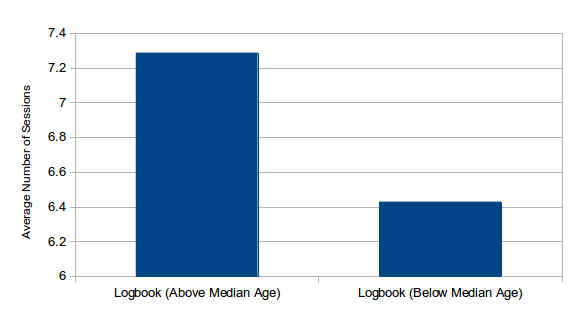
\includegraphics[width=0.5\textwidth]{Figures/logbookbyage.png}
    \rule{35em}{0.5pt}
  \caption{Average number of logbook sessions on  14 intermediaries: Age \textgreater= median age(=15.5) versus Age \textless median age.}
  \label{figure:logbookbyage}
\end{figure}

\begin{figure}[htbp]
  \centering
    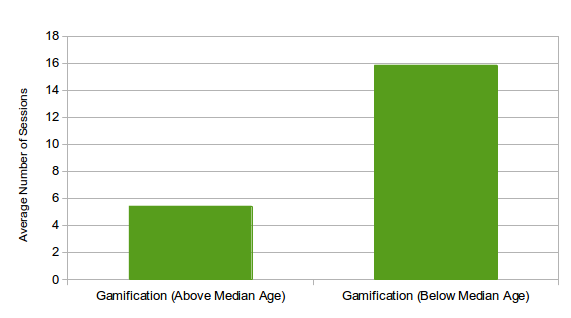
\includegraphics[width=0.5\textwidth]{Figures/gambyage.png}
    \rule{35em}{0.5pt}
  \caption{Average number of gamification sessions on  14 intermediaries: Age \textgreater= median age(=15.5) versus Age \textless median age.}
  \label{figure:gambyage}
\end{figure}

\begin{figure}[htbp]
  \centering
    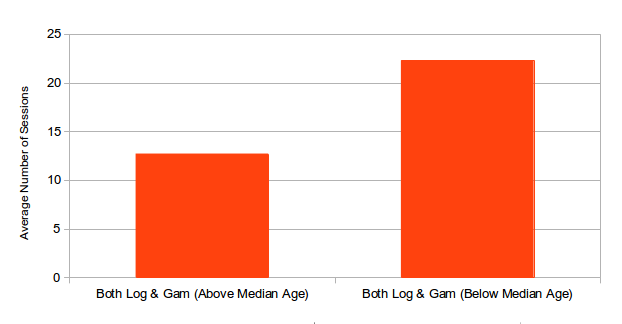
\includegraphics[width=0.5\textwidth]{Figures/bothexpebyage.png}
    \rule{35em}{0.5pt}
  \caption{Average of total number of sessions of  14 intermediaries on both experimental conditions: Age \textgreater= median age(=15.5) versus Age \textless median.}
  \label{figure:bothexpebyage}
\end{figure}
\begin{table}[h!]
  \begin{center}
    \caption{Age groups of intermediary participants}
    \label{table:agregroupsall}
	\begin{tabular}{|c|L{3.2cm}|L{1cm}|L{2cm}|L{2cm}|L{1.6cm}|L{1.3cm}|}
    		\hline
         &\textbf{Age Groups}&\textbf{Total users}&\textbf{No. of GL sequence}&\textbf{No. of LG sequence}&\textbf{No. of Females}&\textbf{No. of Males}\\
         \hline
         1&Age \textgreater=15.5 years&7&3&4&4&3\\  
\hline
         2&Age \textless15.5 years&7&4&3&3&4\\  
\hline
	\end{tabular}
  \end{center}
\end{table}
For pairs who had usage problems on Table \ref{table:usageproblems},three out of four intermediary users were above the median age and one below age. A different trend that excludes the intermediary users that belong in these four pairs still appears to be similar to Figures \ref{figure:logbookbyage} and \ref{figure:gambyage}. For logbook condition, only intermediary users from Pairs A, B were removed as their participation as they terminated their early before switched to logbook condition. Pairs C and D started with Logbook and they participated through logbook conditions despite problems in Pair C since the beginning of experiments. Therefore, the new logbook trend only excluded pairs A, and B (Figures \ref{figure:logbookbyage_mod}). For the gamification condition, we removed pairs A,B,C, and D, as usage problems affected their ability to continue engaging with the app, therefore the new trend on average sessions is shown on Figure \ref{figure:gambyage_mod}.

\begin{figure}[htbp]
  \centering
    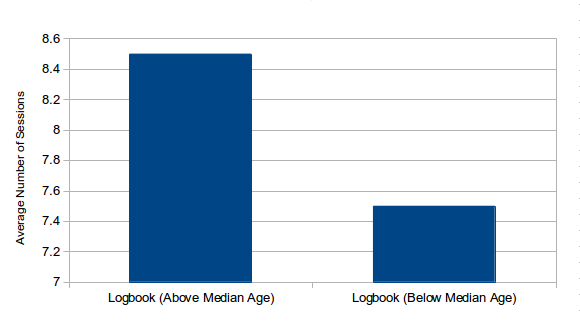
\includegraphics[width=0.5\textwidth]{Figures/logbookbyage_mod.png}
    \rule{35em}{0.5pt}
  \caption{Average number of logbook sessions on  12 intermediaries: Age \textgreater= median age(=15.5) versus Age \textless median age.}
  \label{figure:logbookbyage_mod}
\end{figure}
\begin{figure}[htbp]
  \centering
    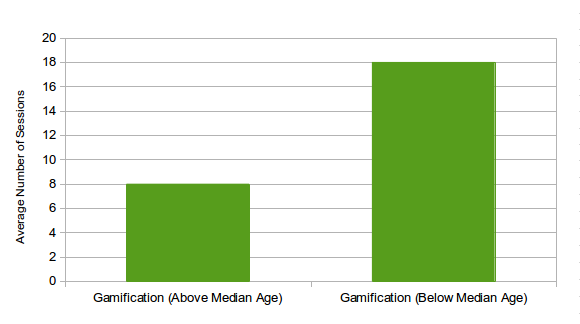
\includegraphics[width=0.5\textwidth]{Figures/gambyage_mod.png}
    \rule{35em}{0.5pt}
  \caption{Average number of gamification sessions on  10 intermediaries: Age \textgreater= median age(=15.5) versus Age \textless median age.}
  \label{figure:gambyage_mod}
\end{figure}
The same trends continue to hold as younger intermediaries appear to have higher average number sessions in gamification condition and lower average number of sessions in logbook condition. \cite{koivisto2014demographic} found that the usage of  a gamified system is highly affected by the novelty effect which is inversely proportional to the age of participants, meaning that highly usage due to the novelty effect may be reported in much younger participants.

The next trend is just looking at usage with respect to both ages of beneficiaries and intermediaries.  If we consider all beneficiary users from all fourteen pairs then the trend on average number of sessions is as shown on Figure \ref{figure:pairs_usage_sessions}. The median age for intermediaries was 15.5 years old while the median age for beneficiaries was 44 years old. Therefore an individual participant belongs to either younger or older group depending on whether ones age is below or above their respective median age. Pairs with a combination of a younger intermediary, and younger beneficiary appears to have more sessions in average. Most of these sessions were contributed by gamification.
 
\begin{figure}[htbp]
  \centering
    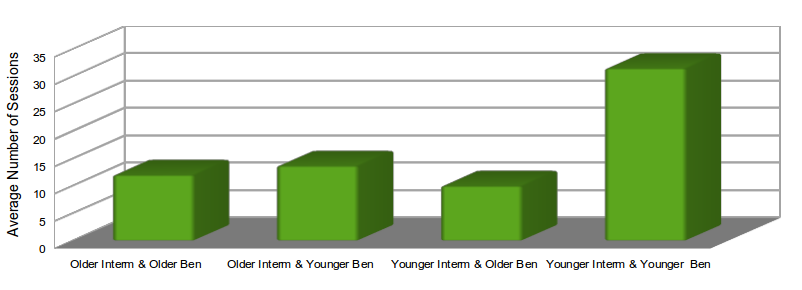
\includegraphics[width=0.6\textwidth]{Figures/pairs_usage_sessions.png}
    \rule{35em}{0.5pt}
  \caption{Average number of sessions on  14 pairs by age groups: intermediaries and beneficiaries}
  \label{figure:pairs_usage_sessions}
\end{figure}
On the next sub sections, user experiences of both intermediaries and beneficiaries are reported.
\subsection{Intermediaries' User Experience}
Most of the time, beneficiaries' usage of the app was facilitated by intermediaries in proximate enabling and proximate translation. These types of intermediated interactions have been discussed in the work by Sambasivan et al.\cite{sambasivan2010}. Baseline data indicated that interest of intermediary participants in using cellphones was higher than that beneficiary participants. For instance, in overall IMI scores to use cellphone, intermediaries (M=5.76, S.D= 0.41, N=14) scored  significantly higher than beneficiary participants (M=5.06, S.D= 0.71, N=13) with (t(25)= 3.1764, p=0.0039, 95\% CI = 0.2472 to 1.1589).

In user experience of intermediaries, the first finding is on how baseline intrinsic motivation and  demographic information such as age of intermediary users influenced user experience. From Figure \ref{figure:bothexpebyage} above, young intermediaries (age\textless median=15.5 years) appeared to had more number of sessions per day on average, but contrary to this trend was that, at baseline the average perceived enjoyment on helping with cellphone related tasks was higher in intermediaries with age\textgreater=median compared to intermediaries with age\textless median for the 12 intermediary users as shown on Figure \ref{figure:PE_HELP_Age}. 
\begin{figure}[htbp]
  \centering
    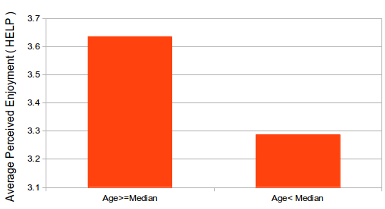
\includegraphics[width=0.5\textwidth]{Figures/PE_HELP_Age.png}
    \rule{35em}{0.5pt}
  \caption{Intermediaries' average perceived enjoyment to help others with cellphone tasks versus age group.}
  \label{figure:PE_HELP_Age}
\end{figure}
The descriptive finding on perceived enjoyment to use the family wellness app by age at midline and endline for the 12 intermediary users (excluding users from pairs A and B since they terminated their usage too soon) showed that the averages are higher on the intermediaries with age \textless median for both midline and endline points (Figure \ref{figure:PE_Interm_App}). If we split the two age groups by, participants with different characteristics are evenly present to both groups as shown on Table \ref{table:agegroups}. Therefore, comparison of trends by age groups in not much influenced by other factors such the experimental sequence of which participants were assigned to or gender. 
\begin{figure}[htbp]
  \centering
    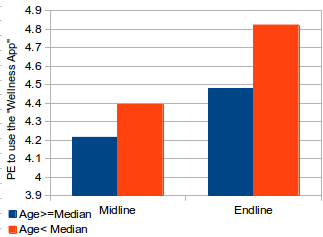
\includegraphics[width=0.5\textwidth]{Figures/PE_Interm_App.png}
    \rule{35em}{0.5pt}
  \caption{Intermediaries' average perceived enjoyment in using the app versus age group.}
  \label{figure:PE_Interm_App}
\end{figure}

\begin{table}[h!]
  \begin{center}
    \caption{Age groups of intermediary participants}
    \label{table:agegroups}
	\begin{tabular}{|c|L{3.2cm}|L{1cm}|L{2cm}|L{2cm}|L{1.6cm}|L{1.3cm}|}
    		\hline
         &\textbf{Age Groups}&\textbf{Total users}&\textbf{No. of GL sequence}&\textbf{No. of LG sequence}&\textbf{No. of Females}&\textbf{No. of Males}\\
         \hline
         1&Age \textless 15.5 years&6&3&3&2&4\\  
\hline
         2&Age \textgreater=15.5 years&6&2&4&4&2\\  
\hline
	\end{tabular}
  \end{center}
\end{table}

The trend on average perceived enjoyment in both logbook and gamified conditions appeared to be slightly higher in younger intermediaries compared to older intermediaries as shown on Figure \ref{figure:PE_Interm_App_exp_seq}. 
\begin{figure}[htbp]
  \centering
    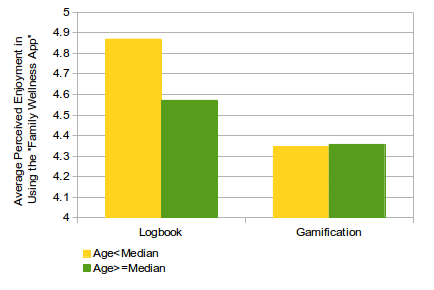
\includegraphics[width=0.5\textwidth]{Figures/PE_Interm_App_exp_seq.png}
    \rule{35em}{0.5pt}
  \caption{Intermediaries' average perceived enjoyment in using the app versus age group (Logbook and Gamification).}
  \label{figure:PE_Interm_App_exp_seq}
\end{figure}

Figures \ref{figure:PE_Interm_App} and \ref{figure:PE_Interm_App_exp_seq}  suggest that the task of helping was more interesting to younger intermediaries due to the existence of the aforementioned motivational affordances.

There several factors that influence intermediaries to use the app and these are:
\begin{enumerate}

\item{\textbf{The phone effect}}: The phenomenon of sharing phones was important in nurturing the relationship between intermediaries and beneficiaries. Parents were lending their phones to their kids to access social media sites and games. Having access to a phone while providing help to beneficiary participants can be viewed as one of the motivating factors to intermediary participants who didn't have smart-phones or data bundles in their smart-phones. Some intermediary participants had installed games, other apps on those phones.

\userquote{\textbf{Siyamthanda}, a female intermediary from Langa, 12 yrs old} {``I had freedom [in using the app] because sometimes she left the phone with me and I was able to play games''}

\userquote{\textbf{Aziza}, a female beneficiary from Athlone, 35 yrs old} {``We would fight over it[the app]. Because he always wants to be on the phone. Always always.''}

\userquote{\textbf{Likhaya}, a male intermediary from Langa, 16 yrs old} {``I didn't feel burdened. You know I also play games on the phone. [Implying he also played games with the phone during logbook condition therefore he didn't feel burdened to help his mother]''}

Therefore, a phone had some effect, since intermediaries were helping in return they have access to cellphone to access functionality or services they like.

\item{\textbf{Gamification comparison}}: The ``Gamified App'' was designed in such a way that a pair will earn rewards based on usage and the average number of steps walked by a beneficiary participant who is a member of the pair. The purpose of rewards was to foster users' intrinsic experiences such as competitiveness and a sense of autonomy which are predictors of intrinsic motivation. Rewards depended on four parameters and these were the number of steps walked by a beneficiary user, the number of days the app has been used by an intermediary to either to record meals or to view feedback on meals, points, steps, gardens, etc. 

Comparison on virtual rewards among intermediaries motivated intermediaries to check the app more often compared to when they were in logbook condition as highlighted on the aforementioned usage findings (sub section \ref{usageoutcome}). Intermediaries were competing which other on the leader board and they talked about their points whenever they meet face to face.

\userquote{\textbf{Jenner}, a female beneficiary from Athlone, 45 yrs old} {``He [Leon (her 15 years old son) ] likes this exercise (using the app) because among him and his friends, they would have that competition like `I got more points than you' and that motivated him to get interested with the app''} 

The competition also led intermediaries to work closer with their beneficiaries.

\userquote{\textbf{Kelvin}, a male intermediary from Athlone, 15 yrs old} {``When I see other people trying to come above me [on the leader board]. I hand over the phone to my mom so she can walk more steps.''} 

\userquote{\textbf{Celine}, a female intermediary from Athlone, 16 yrs old} {``I told my mom that me my self I want our team to have the highest points. Yes she said she is going to do that.''} 

\userquote{\textbf{Sophia}, a female intermediary from Athlone, 17 yrs old} {``Sometimes that person may be first so I tell my mom that we must also be at the first place.[She looks at the  leader board and she sees so and so is at first place there she talks to her mother that they should also aim for the first position] ''} 

\userquote{\textbf{Jenner}, a female beneficiary from Athlone, 45 yrs old} {``When he [Leon] looked through it [The app] and sees their points, he would say `Mom, we need to do something here, because look at their points and our points'. So it was quite interesting.''} 

There was a scenario of one pair of whereby not only the beneficiary was using the pedometer, an intermediary was also taking turns to use the pedometer, therefore they were collaborating in accumulating steps. Both an intermediary user and a beneficiary user had discussions of whether the person whose turn it was had walk enough steps. They did this to accumulate more steps than other pairs. In addition to comparison other intermediary users came to the app to the gamified app to connect to other users.

\userquote{\textbf{Celine}, an intermediary} {``I ask her how far did you walk?  She would say she walked very far. She tells me that I must have the phone to walk more steps. She would say `I got more more walking than you' [They were collaborating with her mother in accumulating steps]. She sometimes writes the steps on the page and she tells me yesterday I day I had more points than you [points referring to steps ]''} 

Rewards were specific for gamification condition by they appeared to also affected pairs that had started with logbook conditions as some intermediary users were pushing their beneficiaries to do more by expecting to get rewards once they are switched to gamification condition.

\userquote{\textbf{Kefiloe}, a female beneficiary from Langa, 26 years old} {``I think we talk more than before the family wellness app. Before the family wellness app, after work it was just ``Hi'' and then I go to my room but now. But now she would come to my room  and say let me see your phone,  what did you eat today,  and write everything down on the phone. So we are more closer than before because of this. Most of the time she used to say that `we must win this'''} 

\item{\textbf{Requests from beneficiary users}}: There were times where intermediary users engaged with the app only upon receiving requests from beneficiaries. In both absence and presence of gamification, intermediaries had to fulfil requests from beneficiaries.  But during logbook condition, intermediaries appeared to be less enthusiastic in handling those requests. Some beneficiaries complained that there were several incidences of where intermediaries were refusing to fulfil these requests and it happened more often during logbook condition. It was observed that in most of these cases, intermediary participants' autonomy was violated as requests came at times where intermediary participants were either studying for exams or doing something else and they felt it was not the right time to fulfil those requests. This made some of the intermediary participants to feel that their parents were nagging them. For instance, \textbf{Lunga}, a male intermediary participant from Langa, aged 17 years, felt annoyed when his mother insisted they should enter the family wellness app while he was busy using social media through the intervention's phone. This happened during logbook condition. Also a similar situation happened to \textbf{Jennifer}, female intermediary participants from Athlone, aged 18 years who also felt irritated by her mother's constant requests during logbook condition. In addition she felt the app was not that exciting as she said ``\emph{The app was okay first but it started to get boring. You don't want to go into it any more. I think there will be some excitement now if the game comes in. When do we get the game}''. She was curious to know when they will be switched to gamification because she thought the logbook condition was boring.

Interest of intermediaries or pairs in general varied as some exhibited interests on interacting with others through the app while others where focused on achievements (i.e. dominating others in competitions). Gamification appeared to be the most dominant factor that influenced usage as we have already seen that the frequency of usage showed a higher value in gamification when compared to logbook. 

\userquote{\textbf{Aziza}} {``We [with Kelvin] were not talking to others because all we wanted was to win. We didn't want them to know but they could see from the app''}
 
Only two intermediaries had tried to interact with others using social features of the app or comment on rewards from their peers. These are some of the comments that were shared by these participants.

\userquote{\textbf{Simon}, a male intermediary from Athlone, 15 yrs old} {``Fish are increasing neh.[He commented this on a fish tank owned by Kelvin and his mother]''} 

\userquote{\textbf{Siyamthanda}, a female } {``Wow it shows that you are working hard  Clara\#2.[She congratulated a female intermediary called Clara for being on the second position on Fish tanks.]''} 

However, not all intermediaries had a positive user experience on utilizing gamification, that is why the average perceived enjoyment appears to be lower for both age groups while in gamification condition compared to the logbook condition (Figure \ref{figure:PE_Interm_App_exp_seq}).

\end{enumerate} 

Leader-board can demotivate those users that are at the bottom but it can foster aspects of relatedness for all users~\citep{sailer2013:psychological}. In this case there were users who never made any advancement in badges hence they appeared at the bottom of the leader board. Some participants it was due to technical problems as reported on Table \ref{table:usageproblems}. But there few exceptions of which two users had no technical problems but never had any advancement in badges despite their efforts in using the gamified system more than the logbook condition as shown on Figure \ref{figure:badge_failure_2}. One user was from the `LG' group (Keller), while the other one was from the `GL' group (Leon).  Their beneficiary participants were not walking enough steps despite the fact that these two intermediaries had put  more efforts in using the app during gamification condition than in logbook condition.
\begin{figure}[htbp]
  \centering
    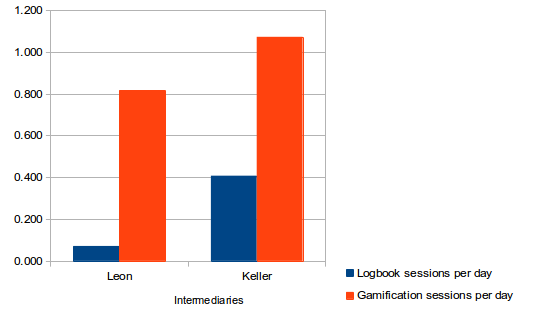
\includegraphics[width=0.7\textwidth]{Figures/badgesfailures2.png}
    \rule{35em}{0.5pt}
  \caption{Logbook Vs Gamification for two users that had no technical problems but never had any badge advancement.}
  \label{figure:badge_failure_2}
\end{figure}

Badges were earned in combination of both the app usage and average number of steps walked by a beneficiary user. One beneficiary who was working with one of these intermediary users also reported in interviews that there was always a contention with her intermediary when this beneficiary wanted to see what was going in the app as the intermediary was not voluntarily willing to help some of the time. It is hypothesized that this could be one of the factors that played a role in demotivating some participants during gamification condition. There were also cases of  where intermediaries doubted the credibility of the system because their peers appeared to be more engaged with the app, but were at lower positions on the leader board. 

\userquote{\textbf{Akhona}, a female intermediary from Langa, 16 yrs old} {``It [The experience in using the gamified app] was the same as last time (during logbook condition) except for the game part. I was actually above some of the others. That was weird. Because they were more interested in the app than me.''} 

On the aforementioned excerpt, \emph{Akhona} was referring to the two intermediaries from pairs C , and D that had usage problem (Table \ref{table:usageproblems}) as these two users used the app more in logbook condition, therefore, Akhona's anticipation was that they would be more competent than her but surprisingly she was ahead of them.  Therefore, even in perceived competence Akhona reported lower score in gamification compared to logbook despite using gamification for 7 out of 14 days and logbook for only 4 out of 27 days.

Therefore, in comparing the support for the three basic psychological needs, pairs that never had any advancement in badges were not considered on aspects of perceived competence and autonomy since majority of them appeared to have a lower perceived enjoyment in gamification when compared to logbook. Autonomy and competence are major predictors of perceived enjoyment. An assumption was that a negative experience was the result of failure of the gamification design to match challenges with abilities. i.e. efforts of beneficiaries differed hence challenges should have matched with individual abilities of beneficiaries within pairs. When challenges are too difficult as they don't match users' skills, end users can become demotivated \citep{zhang2008motivational}. In addition, some of those that had technical problems, their problems were so severe to the extent that they were unable to participate fairly in gamification condition. A total of five intermediary users never had any advancement in badges, therefore, they were excluded in the analysis of motivation of which three are from those that had technical problems (Pairs A, C and D on Table) and two, they had dome more efforts in using the gamified system but there less steps detected from their beneficiaries. As result only nine intermediary users were considered in the perceived competence, and perceived autonomy.

On the aspect of relatedness, all intermediaries were considered because all of them had directly or indirectly use at least one of relatedness features such as receiving SMS showing which teams have advanced in badges, viewing a leader board that shows teams' points, viewing gardens or tanks of different people, and display of badges from each team. These are some of mechanisms to support an aspect of relatedness\citep{sailer2013:psychological}. But in additional, there are intermediary users who knew each other before, and they talked about thinks on the app such as steps comparisons. However there are this that interfered with experiments.     
  
The findings (Table \ref{table:imiwellnessinterm}) indicate that perceived competence of intermediaries in using the ``Family Wellness App'' was significantly higher in the gamified condition than in the logbook condition in the nine intermediaries that were analysed. Perceived autonomy and perceived relatedness were all not different between gamification condition and logbook condition. When I compared perceived autonomy during phase 1 of experiments (at midline point) and during phase 2 of experiments (endline), the perceived autonomy was significantly higher at midline (M=4.44; S.D=0.93) than at endline (M=3.89; S.D=0.76), (t(8)= 2.5298; p=0.0353; 95\% CI= 0.049 to 1.062). Several reasons contributed to this, and these include (1)the learning effect as users became used to the application and the whole exercise was not exciting any more, and (2) most intermediaries were writing exams, and felt that they had no time to do the app, although their beneficiaries kept on pushing them to do the app.

\begin{table}[h!]
  \begin{center}
    \caption{Comparison of ten intermediaries' scores on sub-scales of competence, autonomy, enjoyment, and relatedness in using the ``Family Wellness App}
    \label{table:imiwellnessinterm}
	\begin{tabular}{|c|c|c|}
		\hline
		Mean &Logbook App&Gamified App\\
		\hline
		 \multirow{2}{*}{Perceived competence}&M=5.42; SD=0.88&M=6.03; SD=0.65\\\cline{2-3} 

		 &\multicolumn{2}{|l|}{t(8)=3.1418; p=0.0138 ; 95\% CI= -1.0712 to -0.1643 } \\
\hline
		 \multirow{2}{*}{Perceived autonomy}&M=4.0; SD=0.92&M=4.33; SD=0.84\\\cline{2-3} 

		 &\multicolumn{2}{|l|}{t(8)= 1.2344; p= 0.2521; 95\% CI=  -0.956 to 0.289 } \\
\hline
		 \multirow{2}{*}{Perceived relatedness}&M=4.20; SD=0.59&M=4.5; SD=1.04\\\cline{2-3} 
		 &\multicolumn{2}{|l|}{t(13)= 1.5046; p=0.1563; 95\% CI= -0.725 to 0.13 } \\
\hline
	\end{tabular}
  \end{center}
\end{table}
\subsection{User Experience of Beneficiaries}
As most beneficiaries only interfaced with the app through intermediary users, beneficiaries' user experience relied on cooperation they got from intermediaries. On support for the three basic psychological needs, there was no difference between logbook and gamification. However, aspects of relatedness (N=14) appeared to improve significantly with time when compared between midline (M=4.43; S.D=0.92) and endline (M=5.38; S.D=1.08) with (t(13)= 2.3736; p= 0.0337; 95 \% CI=-1.819 to -0.0855 ). Therefore, the intervention in general made beneficiaries felt more closer at end-line.

On utilizing the app through intermediaries, there are cases where beneficiaries had a negative experience as result of intermediaries refusing to assist upon being given requests. This happened in cases of where intermediary users didn't feel like helping because of being occupies by other tasks such as reading for exams or because they felt the app was boring especially in logbook condition. Younger beneficiaries had a tendency of being keen to compete with others. But for older intermediaries, interests what happening in gamification In addition to that, from Figure \ref{figure:pairs_usage_sessions}, a combination of younger intermediary and beneficiary users had more sessions in average and this is because gamification influenced younger intermediary users to use the app, while it also influenced younger beneficiaries to pass their requests to their respective intermediaries more often. For instance in interviewing one pair that consisted of a younger intermediary and beneficiary users, this pair had highest number of sessions in gamification. In the course of using the app they both exhibited playfulness behaviours in engaging with gamification of whereby they discussed strategies about beating other teams. So every time a beneficiary user from this pair would request her intermediary to open the app so that she can see if they are ahead of other teams.

In the next sub-section, the IMIs in self-monitoring of diet and activity are reported. Four pairs with usage problems (Table \ref{table:usageproblems}) were excluded.
\subsubsection{IMI in Self-Monitoring of Diet}
The results on self-monitoring of diet (baseline, midline, and endline) are shown on Table  \ref{table:imidietbenf}. The Mauchly’s test indicated that the assumption of sphericity was not violated with  $\chi{}$\SP{2}(2)=3.76, p=0.152. The results (N=10) on  ``Self-monitoring of Diet'' shown on Table \ref{table:imidietbenf} were from ``Sphericity Assumed'' output. ANOVA showed that there was a significant difference of average IMI scores on self-monitoring of diet measured at baseline, midline and endline.
\begin{table}[h!]
  \begin{center}
    \caption{Comparison of ten beneficiaries' IMI scores in self-monitoring of diet at baseline, midline and endline}
    \label{table:imidietbenf}
	\begin{tabular}{|L{2.8cm}|L{3.2cm}|L{3.2cm}|L{3.2cm}|}
		\hline
		Mean IMI Score &Baseline&Midline&Endline\\
		\hline
		 %\multirow{3}{*}
		 {Self-monitoring}&M=4.48; SD=1.24&M=5.07; SD=1.19;&M=5.55; SD=0.95\\\cline{2-4} 

		of Diet &\multicolumn{3}{|l|}{F(2,18)=3.787; p=0.042} \\
\hline	\end{tabular}
  \end{center}
\end{table}
A finding from a pairwise comparisons (a paired student t-test) indicated that the IMI score at endline was significantly higher than at baseline (Table \ref{table:imipairwisediet}). There was no significant difference on baseline versus midline and midline versus endline (Tables \ref{table:imipairwisediet1}, and \ref{table:imipairwisediet2}). Motivation to self-monitor diet appeared to increase with time as shown on Figure \ref{figure:imi_diet}. The interpretation of the above findings are that the wellness app appeared to had a significant effect of time on motivation of beneficiaries to self-monitor their diet.
\begin{table}[h!]
  \begin{center}
    \caption{Pairwise comparisons of IMI scores in self-monitoring of diet: Baseline versus Midline}
    \label{table:imipairwisediet}
	\begin{tabular}{|L{2cm}|L{4cm}|L{4cm}|}
		\hline
		Mean &Baseline&Midline\\
		\hline
		 \multirow{2}{*}{IMI Score}&M=4.48; SD=1.24&M=5.07; SD=1.19\\\cline{2-3} 

		 &\multicolumn{2}{|l|}{t(9)=-1.298; p=0.227 ; 95\% CI= -1.621 to 0.439} \\
\hline
	\end{tabular}
  \end{center}
\end{table}
\begin{table}[h!]
  \begin{center}
    \caption{Pairwise comparisons of IMI scores in self-monitoring of diet: Baseline versus Endline}
    \label{table:imipairwisediet1}
	\begin{tabular}{|L{2cm}|L{4cm}|L{4cm}|}
		\hline
		Mean &Baseline&Endline\\
		\hline
		 \multirow{2}{*}{IMI Score}&M=4.48; SD=1.24&M=5.55; SD=0.95\\\cline{2-3} 

		 &\multicolumn{2}{|l|}{t(9)=-2.457; p=0.036 ; 95\% CI= -2.06083 to -0.08517} \\
\hline
	\end{tabular}
  \end{center}
\end{table}
\begin{table}[h!]
  \begin{center}
    \caption{Pairwise comparisons of IMI scores in self-monitoring of diet: Midline versus Endline}
    \label{table:imipairwisediet2}
	\begin{tabular}{|L{2cm}|L{4cm}|L{4cm}|}
		\hline
		Mean &Midline&Endline\\
		\hline
		 \multirow{2}{*}{IMI Score}&M=5.07; SD=1.19&M=5.55; SD=0.95\\\cline{2-3} 

		 &\multicolumn{2}{|l|}{t(9)=-1.975; p=0.08 ; 95\% CI= -1.0342 to 0.07017} \\
\hline
	\end{tabular}
  \end{center}
\end{table}

\begin{figure}[htbp]
  \centering
    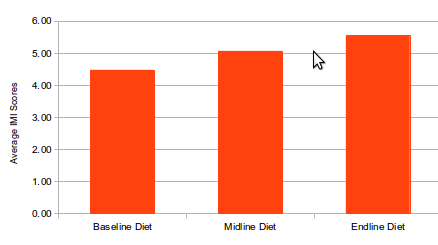
\includegraphics[width=0.4\textwidth]{Figures/imi_diet.png}
    \rule{35em}{0.5pt}
  \caption{Trend on Average IMI Scores of Self-Monitoring of Diet at Baseline, Midline, and Endline.}
  \label{figure:imi_diet}
\end{figure}
The aforementioned ANOVA finding on comparison among baseline, midline, and endline doesn't discern between different experimental conditions of which pairs of users were exposed to. The ANOVA finding (N=10)(Table  \ref{table:imidietbenf2}) on the comparison of IMI scores to self-monitor diet, among baseline, logbook, and gamification conditions showed that there was no significant difference of average IMI scores on self-monitoring of diet measured during baseline, logbook and gamification conditions. This finding is from the ``Sphericity Assumed'' output of the ANOVA test since the Mauchly’s test indicated that the assumption of sphericity was not violated with  $\chi{}$\SP{2}(2)=2.19, p=0.335. The trend on averages shows both logbook and gamification to be slightly higher than baseline as shown on Figure \ref{figure:imi_diet2}. The conclusion from this finding is that both versions of the prototype have shown an indication of increasing motivation of beneficiaries to self-monitor diet.
\begin{table}[h!]
  \begin{center}
    \caption{Comparison of ten beneficiaries' IMI scores in self-monitoring of diet at baseline, after logbook, and  after gamification conditions}
    \label{table:imidietbenf2}
	\begin{tabular}{|L{2.8cm}|L{2.5cm}|L{2.5cm}|L{2.5cm}|}
		\hline
		Mean IMI Score &Baseline&Logbook&Gamification\\
		\hline
		 %\multirow{3}{*}
		 Self-monitoring&M=4.48; SD=1.241&M=5.28; SD=1.05&M=5.34; SD=1.16\\\cline{2-4} 
		 of Diet&\multicolumn{3}{|l|}{F(2,18)=3.787; p=0.087} \\
\hline	\end{tabular}
  \end{center}
\end{table}
\begin{figure}[htbp]
  \centering
    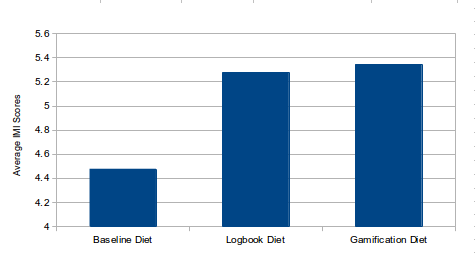
\includegraphics[width=0.4\textwidth]{Figures/imi_diet2.png}
    \rule{35em}{0.5pt}
  \caption{Trend on Average IMI Scores of Self-Monitoring of Diet at Baseline, Logbook, and Gamification.}
  \label{figure:imi_diet2}
\end{figure}
\subsubsection{IMI in Self-Monitoring of Activity}
The results (N=9) on self-monitoring of activity are shown on Table  \ref{table:imiactivitybenf}. The results are based on a sample of nine beneficiary users as one participant didn't complete this part of the questionnaire at baseline.  The Mauchly’s test indicated that the assumption of sphericity was violated with  $\chi{}$\SP{2}(2)=8.248, p=0.016. The value $\epsilon$ on Greenhouse Geisser was ``\textless 0.75'', therefore, the results on  ``Self-monitoring of Diet'' shown on Table \ref{table:imiactivitybenf} were selected from ``Greenhouse-Geisser'' output. ANOVA showed that there was no significant difference of average IMI scores on self-monitoring of activity measured at baseline, midline and endline. The trend of means appears to increase from baseline to endline as shown on Figure \ref{figure:imi_activity}.

There are several factors that could have contributed to results not being significant among baseline, midline,endline points,. The first hypothesized reason is tracking of physical activity appeared to be easy in majority of the participants even without tracking devices as people can estimate the distance they walk daily and they consider this as tracking even though they might have means to record this information, hence their motivation was high at baseline unlike diet self-monitoring which they consider it to be cumbersome due to external barriers such as health food being expensive, therefore at baseline participants felt more motivated to track their activity. The second hypothesized reason is that the sample size was small hence there was a smaller power in detecting significant difference. But we have seen that the trend in motivation increases with time.
\begin{table}[h!]
  \begin{center}
    \caption{Comparison of ten beneficiaries' IMI scores in self-monitoring of activity at baseline, midline and endline}
    \label{table:imiactivitybenf}
	\begin{tabular}{|L{2.8cm}|L{2.5cm}|L{2.5cm}|L{2.5cm}|}
		\hline
		Mean IMI Score &Baseline&Midline&Endline\\
		\hline
		 %\multirow{3}{*}
		 Self-monitoring&M=4.82; SD=1.002&M=5.28; SD=1.003&M=5.41; SD=0.894\\\cline{2-4} 
		 of activity&\multicolumn{3}{|l|}{F(1.182, 9.455)=2.936; p=0.116} \\
\hline	\end{tabular}
  \end{center}
\end{table}

\begin{figure}[htbp]
  \centering
    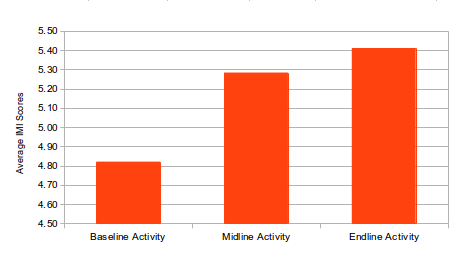
\includegraphics[width=0.4\textwidth]{Figures/imi_activity.png}
    \rule{35em}{0.5pt}
  \caption{Trend on Average IMI Scores of Self-Monitoring of Activity at Baseline, Logbook, and Gamification.}
  \label{figure:imi_activity}
\end{figure}
The finding from an analysis (N=9) that examined if there is a difference among baseline,logbook, and gamification in self-monitoring of activity, showed that there was no significant difference of average IMI scores on self-monitoring of activity measured at baseline, logbook and gamification (Table {table:imiactivity2benf}). The Mauchly’s test indicated that the assumption of sphericity was violated with  $\chi{}$\SP{2}(2)=6.788, p =0.034. The value of $\epsilon$ on Greenhouse Geisser was ``\textless 0.75'', therefore, these results on  ``Self-monitoring of Activity'' were selected from ``Greenhouse-Geisser'' output of oen way with repeated measures ANOVA test. The trend in motivation increases in both logbook and gamification compared to baseline as shown on Figure \ref{figure:imi_activity2}
%epsilon=0.617
\begin{table}[h!]
  \begin{center}
    \caption{Comparison of ten beneficiaries' IMI scores in self-monitoring of activity at baseline, logbook and gamification}
    \label{table:imiactivity2benf}
	\begin{tabular}{|L{2.8cm}|L{2.5cm}|L{2.5cm}|L{2.5cm}|}
		\hline
		Mean IMI Score &Baseline&Logbook&Gamification\\
		\hline
		 %\multirow{3}{*}
		 Self-monitoring&M=4.82; SD=1.002&M=5.33; SD=0.9762&M=5.37; SD=0.9276\\\cline{2-4} 
		 of activity&\multicolumn{3}{|l|}{F(1.234, 9.872)=2.783; p=0.123} \\
\hline	\end{tabular}
  \end{center}
\end{table}
\begin{figure}[htbp]
  \centering
    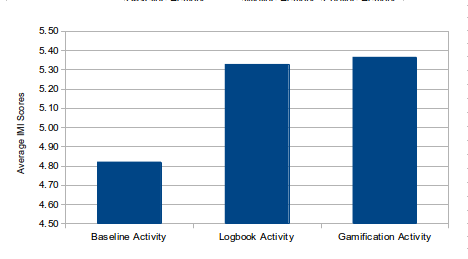
\includegraphics[width=0.4\textwidth]{Figures/imi_activity2.png}
    \rule{35em}{0.5pt}
  \caption{Trend on Average IMI Scores of Self-Monitoring of Activity at Baseline, Logbook, and Gamification.}
  \label{figure:imi_activity2}
\end{figure}
\section{Discussion}
In many cases, usage of the app was controlled by intermediaries. Intermediaries engaged with the app mostly because of two factors and these were: either competitions with others or request from their beneficiaries. Beneficiaries interests varied and it was influenced by  either one of the following factors or both: (1) leader board; and (2) instrumental value provided by the app. Not all beneficiaries were motivated by gamification. However, gamification was the main source of motivation to intermediaries and it played a pivotal role in mediating usage. Gamification also mediated intermediaries to influence or persuade their beneficiaries.  For instance, in one scenario a beneficiary described how serious her son was engaged in competition with others and was always reminding her to carry the pedometer whenever she wants to go out as shown on the following excerpt.

\userquote{\textbf{Jenner}, a female beneficiary from Athlone, 45 yrs old} {``Sometimes may be I forget to take the phone when I go walking and he would ask me `did you take the phone with you' Ooh Gosh I forgot.  Because when I walk to Park Town to exercise and sometimes  I am in such a hurry I forget the phone, he will be crossed with me. ''} 

For intermediaries that started with logbook, majority of those that engaged with logbook many times did with an interest of winning the competition once switched to gamification. Therefore, this affected the separation of experimental as users were aware that they will be switched to gamification at some point. For the case of perceived competence, the difference between logbook and gamification was statistically significant and intermediary user in gamification felt more competent.Statistical significance in difference was not achieved in cases of autonomy and relatedness due to the learning effect and a smaller sample size. 

Apart from gamification, another important source of motivation that can be leveraged is, beneficiaries' phones. Beneficiaries were custodians of intervention's phone. But in many cases when beneficiaries were at home they left the phone with the intermediaries who were interested with social media sites and  games. Intermediaries were interested with those phones because of either of the two reasons or both: (1) Interventions phone's were better than intermediaries' phones or intermediaries didn't have smart phones that can enable to access services they desire; and (2) Availability of data bundles in intervention's phones through inserted SIM cards. In these scenarios, some intermediaries were implicitly reciprocating the favours of having freedom to use the phone by serving requests from their beneficiaries. In the context of ICTD, non-prescribed use of devices or other technologies allocated for an intervention is considered to be an aspect of play which is a capability as it fosters motivation to participate in an intervention \citep{ferrplay2015}. Therefore, one can capitalize on this motivation introduced as the result of sharing phones and it can be viewed as part of motivational affordances to encourage ongoing use of a system through young intermediaries within family settings. Utilization of the motivational effect of the phone in mediating such an intervention depends on interest of beneficiaries on the intervention. Without requests from beneficiaries, and with absence gamification on the app for intermediaries, the phone effect itself cannot mediate usage of the app unless it goes in parallel with those two mediating factors for usage.

Gamification was the most dominating motivational affordance. However, there are some factors that need to be taken into considerations in design of gamification in order to curb negative experiences which appeared to harm intrinsic motivation of some intermediary users. Awarding virtual rewards to intermediary users based on partial efforts from beneficiary participants seemed not to resonate with the notion of matching challenges to skills of the main users. For instance in awarding badges there were two conditions to be met. The first condition was that the app has to be used for a certain minimum number of days as specified by requirements of a specific badge. The second condition was that, an average number of steps that have been walked so far has to be not below a certain threshold for that specified badge. It became impossible for some intermediary users to move from one badge to the next because efforts by beneficiary users differed and this may impacted motivation of intermediary participants and this harmed their intrinsic motivation. When challenges are too difficult as they don't match users' skills, end users can become demotivated \citep{zhang2008motivational}. 

Another shortcoming observed in the app, is that the gamified system didn't give users much autonomy apart from only configuration of avatars and editing of profiles. For instance, freedom to select the level of gamification appropriate to the skills they possess at a particular moment was not supported in the app. Examples of ways on which autonomy is supported include profiles, avatars, macros,configurable interface, alternative activities, privacy control, etc. \citep{francisco2012analysis}. 

One of the approaches that could be used to minimize the effect of the  aforementioned shortcomings is to give users more autonomy to select different levels of gamification they want to participate. There could be levels such as beginners, intermediate, advanced, etc. Pairs that are on the same level could be grouped together and not mixed with pairs with levels that are different. In addition, users could be allowed to select which features they would like to include in their interfaces from a range of features such as chat rooms, leader-boards, botanical gardens etc. More autonomy can also be given in customization of privacy in terms of whether they would like to share their information or not. Customization of avatars is also important because It was observed that most users changed their avatars during gamification and one user explained that she sees the avatar she selected as a representation of herself. Through avatars, these users embodied their identities.
 
A different approach in increasing engagement of intermediary users is  to allow intermediary participants to participate with their information, by incorporating their wellness data i.e. steps. The former can also be combined with the latter. There were some observed scenarios that support the utilization of the latter approach. For instance, there was one pair of whereby not only the beneficiary participant was using the pedometer as an intermediary was also using it. They were taking turns to use the pedometer, therefore, they were collaborating in accumulating steps. This pair had discussions of whether the person whose turn it was had walked enough steps. The goal was to accumulate more steps than other pairs. A similar concept has been explored with participants in a low income neighbourhood in USA , of whereby there is an exergame that encourages cooperation between parents and children~\citep{saksono2015spaceship}.

Also another way of increasing engagement is the one reflected by intermediaries who claimed to also be benefiting from nutrition/diet information since the same type of meal is shared at home, therefore, if beneficiary participants ate something that is not healthy while at home then there is a likelihood of an intermediary participant to have eaten the same type of meal too. Also literature suggests that parents who live a healthily lifestyle are likely to also influence their children to live healthily~\citep{grimes2009toward}. Therefore, by creating a system that allows intermediaries to also benefit from usage one can foster internalization through identified and integrated regulations which are somehow close to intrinsic motivation  as these intermediaries are going to put more value to the system because of its perceived benefits. 

  

\begin{flushright}
\end{flushright}

